\begin{enumerate}[label=\thesubsection.\arabic*.,ref=\thesubsection.\theenumi]
    \numberwithin{equation}{enumi}
    
    \item Sketch the Bode magnitude and phase plots for 
    \begin{align}
        G(s) = \frac{\brak{1+0.2s}\brak{1+0.025s}}{s^3\brak{1+0.005s}\brak{1+0.001s}}
    \end{align}
    Also compute the gain margin and phase margin.\\
    \solution
    \begin{align}
        G\brak{j\omega} = \frac{\brak{1+0.2j\omega}\brak{1+0.025j\omega}}{-j\omega^3\brak{1+0.005j\omega}\brak{1+0.001j\omega}}
    \end{align}
    
    Zeros: -5, -40
    
    Poles: 0, 0, 0, -200, -1000
    
    For definitions of phase margin and gain margin, refer to the sections 2.2 and 2.3.
    
    \begin{figure}[!h]
    \centering
      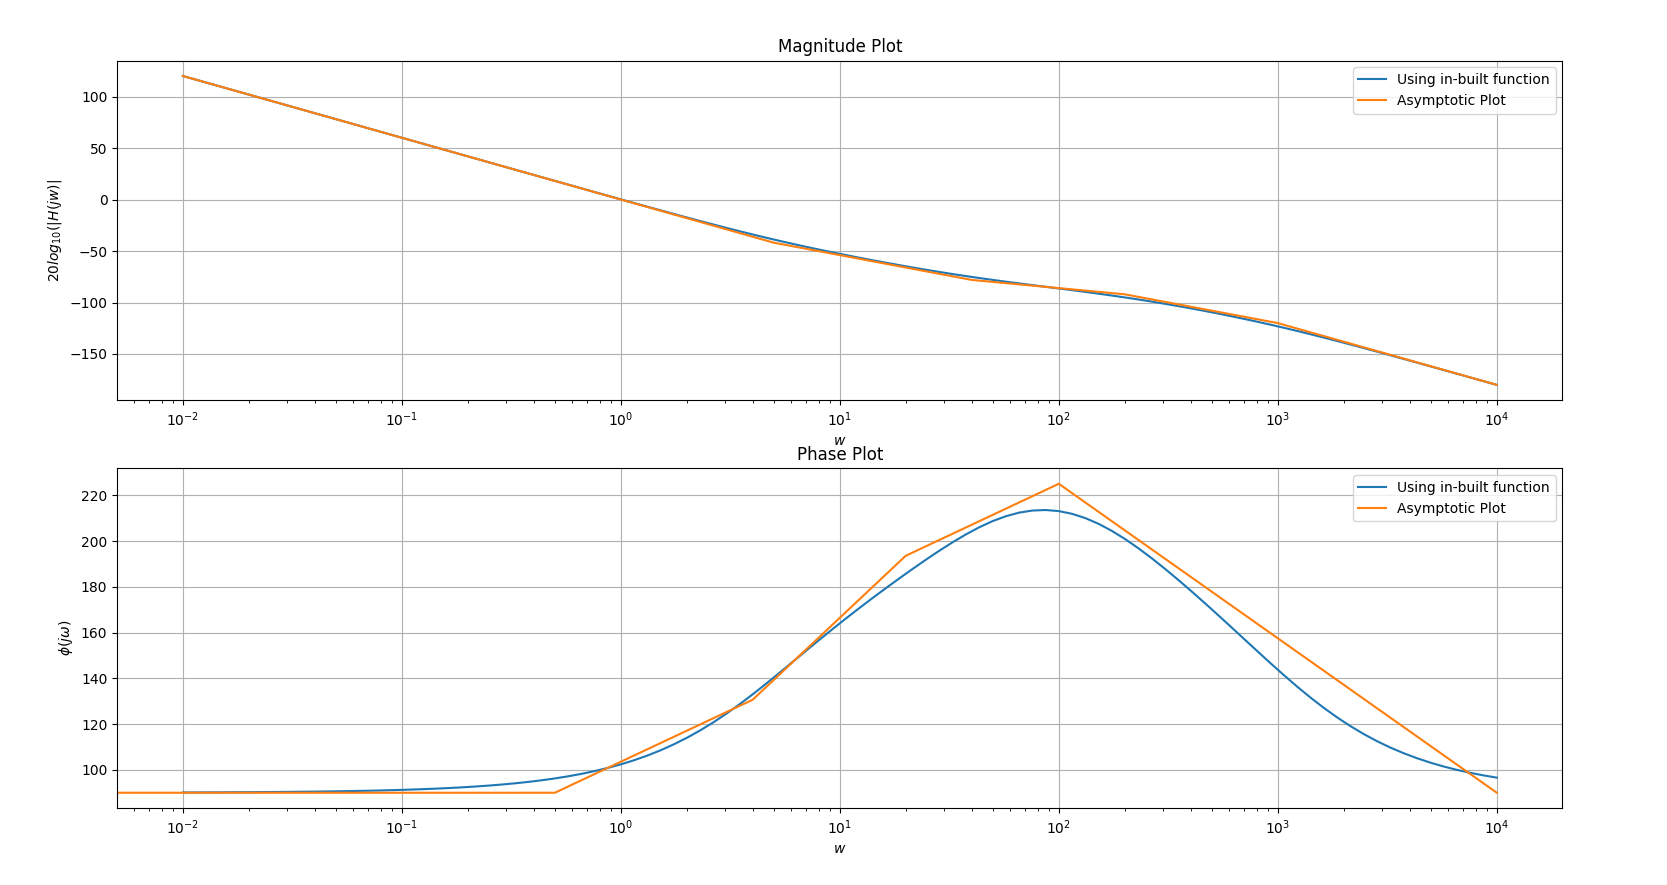
\includegraphics[width=\columnwidth]{bode_plot.png}
      \caption{Bode plot}
      \label{fig:ee18btech11039}
    \end{figure}
    
    Solving (using the plot)
    \begin{align}
        \frac{\sqrt{1+\brak{0.2\omega}^2} \sqrt{1+\brak{0.025\omega}^2}}{|\omega|^3 \sqrt{1+\brak{0.005\omega}^2} \sqrt{1+\brak{0.001\omega}^2}} = 1
    \end{align}
    We get the gain cross-over frequency as \\ $\omega _{gc} = 1$. 
    Computing 
    
        \begin{multline}
            \phase{G\brak{\j\omega_{gc}}} = \tan^{-1}\brak{0.2\omega_{gc}}+\tan^{-1}\brak{0.025\omega_{gc}}+90^0\\
            -\tan^{-1}\brak{0.005\omega_{gc}}-\tan^{-1}\brak{0.001\omega_{gc}}
            = 102.4^0
        \end{multline}
    
    \begin{align}
    \text{Phase Margin, } \phase{G\brak{\j\omega_{gc}}} = 282.4^0
    \end{align}
    
    In the phase plot, $\phi(j\omega)$ reaches $180^0$ at $\omega_{pc} = 16.29$. From fig. \ref{fig:ee18btech11039}, 
    \begin{align}
        20log_{10}\brak{|G\brak{j\omega_{pc}}|} = -61.436 dB
    \end{align}
    The program for plotting bode plot and finding phase margin and gain margin -
    \begin{lstlisting}
        codes/ee18btech11039/bode_plot.py
    \end{lstlisting}
    
    \end{enumerate}
    
    